\section{Purpose of the project - Constructing a matrix}
Now we are ready to describe the scan mathematically. 
First off, the subject is modelled by a grid and each photon beam by a line. 
The angle of a particular emission is denoted by $\sigma$ and the number of parallel lines is denoted $n$. Now the $i$'th line of some angle $\sigma'$ can be written as $(\sigma', i)$. Note that the offset between each line must be known. Let this distance be denoted by $\delta$. The energy upon exit is stored in a vector of size $m$, denoted $\mathbf{y}$.\\

Then, for each of the $m$ angles ($\sigma$s) a discretization of the $n$ lines is needed. This is done by dividing each line into the segments between its intersections with the grid. In particular the length of these segments should be computed, as they are used to approximate the integral that describes the attenuation of that line. For each line, a matrix with the same size as the grid should be produced. At the general entry $(i,j)$ this matrix should have the length of a line segment if the line intersects the corresponding cell in the grid, otherwise zero. This results in a total of $n$ matrixes per emission. 
Let the collection of these $n$ matrixes form a row the matrix $\mathbf{A}$, giving a total of $m$ rows. We are now ready to write the actual problem:
$$
  \text{argmin}_{\mathbf{x}} ~~ || \mathbf{Ax} - \mathbf{y} ||^{2}
$$
Here $\mathbf{x}$ denotes the attenuation constants, and is of length $m$.
While approximating $\mathbf{x}$ is the overarching goal, the main task in this project will be to construct the $\mathbf{A}$ matrix in a fast manner.

\begin{figure}[H]
  \centering
  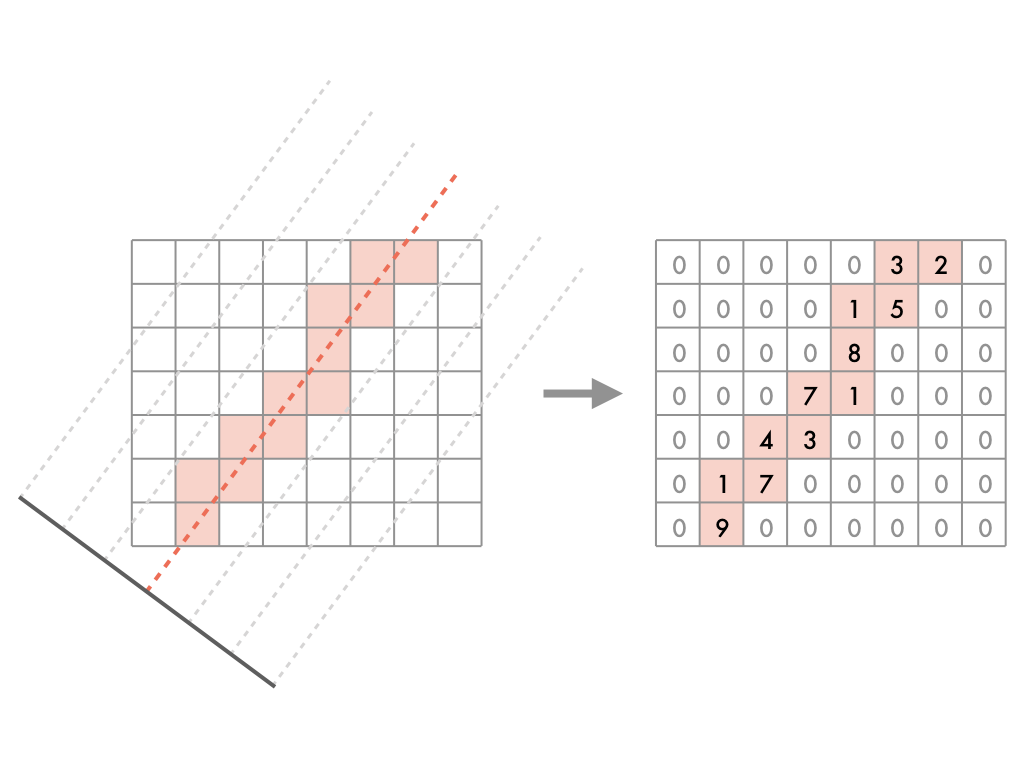
\includegraphics[scale=0.35]{figures/line2matrix.png}
  \caption{A simplified illustration of the discretization of a single line. Note that the intersection lengths should be real numbers instead of integers in a real world setting.}
\end{figure}